\documentclass[12pt]{article}
\usepackage[hidelinks]{hyperref}
\usepackage[square,sort,comma,numbers]{natbib}
\usepackage{graphicx}
\usepackage{booktabs}
\title{Improving Speed and Interestingness of Graph-Based Specification Mining via Corpus Filtering}
\author{
    Andrew Mason\\
    \texttt{ajm188@case.edu}
    \and
    Jon Pfeil\\
    \texttt{jwp69@case.edu}
}
\date{December 8, 2014}
\begin{document}
\maketitle
\tableofcontents
\pagebreak

\section{Introduction}
Software verification, the ability to prove the correctness of a piece of software \cite{FormalSoftwareVerification}, is an appealing approach to improving software quality. However, the requirement of having formal descriptions of correctness has prevented the widespread use of software verification \cite{Ammons:2002:MS:503272.503275}. \textit{Specification Mining}, as described in \cite{Ammons:2002:MS:503272.503275}, is the machine learning approach to discovering formal specifications for a program interface or an abstract data type. A specification mining tool would reduce the major barrier to program verification by automating the generation of formal specifications.

Our project aims to push forward the current state of specification mining through the application of frequent subgraph mining algorithms to novel intermediate representations of programs.

\section{Background}
\subsection{Software Verification}
Knowing that a software system fulfills a set of requirements correctly is an
important concern in industry, especially for mission-critical software
systems, such as the avionics software in an airplane, or the software in
medical devices. Approaches to software verification can be separated into
categories, dynamic approaches and static approaches.
\\

\noindent Dynamic approaches to software verification include unit testing,
integration and system testing, and acceptance testing. While these methods 
can identify bugs in the software and help improve software quality, alone they
cannot confirm that the system is bug free and that the system fulfills all of
its requirements. A requirement may not be exercised by the tests, and there
may be a bug that occurs only on a particular input which the test suite does
not include.
\\

\noindent We prefer instead the static methods of software verification, known
also as program analysis or formal verification. These techniques aim to
provide a formal proof that a system satisfies a specified property. Numerous
approaches to formal verification exist, and we briefly highlight a few of
them below.
\\

\noindent Model-based certification aims to provide formal proofs that an
abstract model, such as a formal computational model, representing the software
system has a particular property\cite{FormalSoftwareVerification}. In this
approach, a verifier uses a model-checking tool to explore the state space of
the program, searching for error states, states where a certain property of the
system does not hold. One issue with this approach is that the state space for
even trivial programs can grow quite large, but predicate abstraction can be 
used to systematically reduce the state space\cite{FormalSoftwareVerification}.
\\

\noindent Deductive software proving, also referred to as program proving, aims
to express the correctness of a program as a set of mathematical statements,
which are then discharged using a theorem prover
\cite{DeductiveSoftwareVerification}. To do this, a formal specification
language must be defined and integrated with the desired programming language.
Filliâtre claims that the best method for achieving this is to tighten a
specification language to a programming language within a dedicated program
logic, which mixes programs and logical statements, infusing program
contstructs with logical ones in a single language
\cite{DeductiveSoftwareVerification}.

\subsection{Specification Mining}
Formal software verification has the potential to replace testing as the
standard method of verifying program correctness. However, formal program
verifiers are limited in that they can only check specified properties.
Additionally, authors Lo and Khoo claim that the difficulty in formulating a
set of formal properties has contributed to the lack of widespread adoption in
industry\cite{Lo_softwarespecification}. To solve this issue, the technique of
specification mining aims to discover non-trivial properties or specifications
in a software system to later be used by a program verifier.
\\

\noindent Several approaches to specification mining are described in the
literature, the first of which is a machine learning approach outlined by
Ammons et al. Their mining approach is based on program execution traces rather
than static analysis of source code. Ammons et al argue that this approach is
superior since the traces will only contain the feasible paths of execution.
Additionally, basing the mining on program traces ensure that only correct
execution paths are mined, thus preventing buggy paths from polluting the
results of the mining\cite{Ammons:2002:MS:503272.503275}. Their miner extracts
abstract scenarios from traces annotated with information about flow
dependence, which are small sets of independent interactions. These scenarios
are then fed into an automaton learner to learn the specifications. Ammons et
al give two reasons for this approach. First, the scenarios are much smaller
than the original traces, so the automaton learner learns the specifications
much faster. Second, the sizes of the scenarios are bounded, which they argue
make the specification mining tractable. The workflow of the miner looks like
\cite{Ammons:2002:MS:503272.503275}:\\
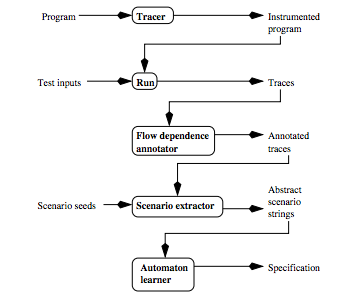
\includegraphics{machine_learning_miner_workflow.png}
\\

\noindent Lo and Khoo expand on the work of \cite{Ammons:2002:MS:503272.503275}
by describing their work in automaton-based specification mining, as well as
their work in mining Linear Temporal Logic (LTL) expressions and Live Sequence
Charts (LSC), which are alternate formalisms for representing specifications
\cite{Lo_softwarespecification}. Their approach also relies on execution traces
of the program. Lo and Khoo improve on \cite{Ammons:2002:MS:503272.503275} by
using a data mining approach that attempts to improve the quality of results,
since Ammons et al rely on the notion that traces give strong hints about
program rules, but do not really address the possibility that these traces may
contain errors. To this end, Lo and Khoo add an accuracy metric to measure the
performance of an automaton-based miner, which is measured by the notion of
recall and precision. They define recall and precision as ``the proportion of
sentences in $S_{inf}$ that is accepted by $S_{orig}$ and the proportion of
sentences in $S_{orig}$ that is accepted by $S_{inf}$ where $S_{orig}$ is the
original specification and $S_{inf}$ is the inferred specification
\cite{Lo_softwarespecification}.'' Next, the authors devise a framework they
call SMArTIC that splits the specification mining task into four pipelined
components. They claim that this improves the quality of the mining because it
identifies and filters out erroneous traces early in the mining, and ``the
over-generalization that occurs at the learning stage can be mitigated by
localization of the learning process to groups of related ... traces
\cite{Lo_softwarespecification}.''
\\

\noindent Lo and Khoo also discuss their work in LTL specification mining,
which is one of the most commonly-accepted formalisms by standard verifiers.
LTL expressions break automata-based specifications (which are global and
often complex) into smaller pieces which express what the authors call
strongly observed behavior or rules. To identify these rules, Lo and Khoo
introduce the notions of support, which is the number of traces exhibiting the
premise of the rule, and confidence, which is the likelihood of the premise of
the rule to be followed by its consequence\cite{Lo_softwarespecification}.
They employ a search space pruning strategy to mine these rules from the
execution traces.

\subsubsection{Limiting False Positives}
Le Goues and Weimer\cite{Goues:2009:SMF:1532891.1532925} claim that
specification inference techniques suffer from 90-99\% false positive rates,
and thus require a heavy burden of manual inspection, making these techniques
impractical for most software projects. By defining the notion of code
trustworthiness, they are able to achieve false positive rates of only 5\%.
Their approach statically estimates the trustworthiness of each code fragment
and then weights the contribution of each trace by its trustworthiness, which
is determined by the trustworthiness of the fragments visited in the trace, in
the actual specification mining\cite{Goues:2009:SMF:1532891.1532925}. The code
trustworthiness is based on the notion that some code is more likely to be
correct than others. Le Goues and Weimer estimate this likelihood by using the
results of many studies in software engineering. For example, studies have
shown that code that is modified more frequently is more likely to contain
defects, so the approach looks at information obtained from the version control
system to determine the rate of what the authors call code churn
\cite{Goues:2009:SMF:1532891.1532925}.

\subsection{Graphical Specification Mining}
\subsubsection{Program Dependence Graphs}
Several techinques have been described in the literature that perform
specification mining on an intermediate representation of the software known
as a procedure dependence graph (PDG). A PDG combines the information contained
in a data dependence graph and a control flow graph. For more information, see
\cite{Ferrante:1987:PDG:24039.24041}.

\subsubsection{Subgraph Isomorphism}
Finding repeated patterns in the PDGs is central to the ideas behind graphical
specification mining, and, therefore, so is the subgraph isomorphism problem.
The subgraph isomorphism problem asks the question: given graphs $G$ and $H$,
does there exist a subgraph $G_0$ of $G$ such that $G_0$ is isomorphic to $H$?
Such an isomorphism is illustrated in the following diagram (C highlights the 
subgraph of B that is isomorphic to A):
\begin{center}
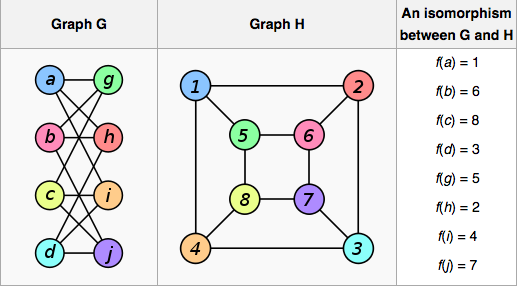
\includegraphics{subgraph_isomorphism.png}
\end{center}

\subsubsection{Frequent Subgraph Mining}
Another fundamental technique in graphical specification mining is that of
frequent subgraph mining. Given a graph dataset
$D = \left\{ G_0, G_1, \ldots, G_n\right\}$, with $support(g)$ denoting the
number of graphs in $D$ in which $g$ is a subgraph, frequent subgraph mining
aims to find all subgraphs $g$ such that $support(g) \geq minSup$, where
$minSup$ is some minimum support, usually specified by a user
\cite{Yan:2002:GGS:844380.844811}. At the heart of frequent subgraph mining is
the subgraph isomorphism test.

\subsubsection{gSpan}
\noindent Yan and Han present an algorithm for mining frequent substructure
patterns, which they call gSpan. It is important to note that the authors
limit their discussion to frequent connected subgraphs only. gSpan explores
depth-first search (DFS) in frequent subgraph mining, introducing the concepts
of DFS lexicographical ordering and a minimum DFS code, which provide a
canonical labeling system to support DFS searching during the mining.
Definitions for these concepts can be found in
\cite{Yan:2002:GGS:844380.844811}. The subgraph mining subroutine of the
algorithm uses a recursive graph expansion strategy, growing the current
subgraph by one edge at a time to find the largest possible subgraph which is
still a frequent subgraph.

\subsubsection{CloseGraph}
\noindent Yan and Han expand upon their work on gSpan in their paper
``CloseGraph: Mining Closed Frequent Graph Patterns.'' They propose a new
algorithm which mines only closed frequent subgraph patterns, rather than all
of them. A graph $g$ is closed if there exists no proper super-graph with the
same support as $g$ \cite{Yan:2003:CMC:956750.956784}. This approach addresses
the issue in gSpan of the blowing up of frequent subgraphs. For example, an
$n$-edge graph has at most $2^n$ subgraphs, which contribute no new
information if they have the same support as the super-graph. Yan and Han
postulate that their approach, CloseGraph, both drastically reduces the number
of unnecessary graphs generated as well as significantly improves the
efficiency of the mining\cite{Yan:2003:CMC:956750.956784}. Their algorithm
makes use of some of the properties of gSpan, in particular DFS coding and
lexicographical ordering, and the restriction of graph extensions to right-most
extensions only, and defines the notion of equivalent occurence (see
\cite{Yan:2003:CMC:956750.956784}) to provide conditions for early
termination. Additionally, Yan and Han show that CloseGraph does not need to
store previously discovered graphs to prune newly discovered non-closed graphs
\cite{Yan:2003:CMC:956750.956784}. Finally, they show that CloseGraph can be
used with minimal effort to mine other structures, including many other types
of graphs (unlabeled, non-simple, directed, and disconnected) as well as trees.
\\

\section{Previous Work}
\subsection{Definitions}
\subsubsection{Graph Minors}

\subsubsection{Dependence Spheres}
\subsection{GMFMM}
\noindent Frequent subgraph mining is an important problem in the field of
specification mining, as these specifications can be modeled by graph minors
of PDGs. Hence, mining the PDG for graph minors results in the discovery of
program specifications. In their paper, ``Discovering program rules and
violations by mining interprocedural dependencies,''
\cite{DBLP:journals/smr/ChangP12} Chang and Podgurski give an approach for
mining maximal frequent minors from interprocedural dependence spheres. By
extending the scope of the minor to an interprocedural level, two additional
types of program specifications can be learned by this approach: rules about
the ordering of function calls, and rules regarding the inputs and return
values of functions. The authors define the notion of maximal frequent
subgraphs to be those which are not contained in any other frequent subgraphs.
Note that this notion is identical to the notion of a closed graph defined in
\cite{Yan:2003:CMC:956750.956784}. Rather than mining all frequent subgraphs,
the approach looks only for frequent minors (see
\cite{DBLP:journals/smr/ChangP12} for a definition of a graph minor), which
allows for certain variations in the structure of certain rules can be
encompassed by a single rule.
\\

In order to mine for interprocedural rules, the authors give an approach for constructing a interprocuderal dependence sphere. The approach begins with the call-site graph (CSG), $S$, of the function of interest, $f_b$. Then, $S$ is grown iteratively by adding nodes from PDGs of functions in the call tree of $f_b$ if there exists a direct data dependency between the node and any node in $S$. See \cite{DBLP:journals/smr/ChangP12} for more details. Since Chang and Podgurski focus on the ordering and conditional rules unique to interprocedural analysis, they offer a method to reduce the resulting intereprocedural dependence sphere to include only call-site graph nodes and control point nodes. It is not difficult to extend the idea behind this reduction to limit the scope of the dependence sphere to any subset of node types that are of interest to the user in order to improve the efficiency of the mining algorithm.

\section{Tools}
\label{section:Tools and Data Sources}
\subsection{Soot}
Soot is a Java optimization framework, intended to be used as either a stand-alone tool to inspect class files, or to develop optimizations or transformations on Java byte code. Soot provides several different intermediate representations of Java byte code: 

\begin{itemize}
    \item\textbf{Baf}: a streamlined representation of bytecode which is simple to manipulate.
    \item\textbf{Jimple}: a typed 3-address intermediate representation suitable for optimization. This is the primary representation used by Soot.
    \item\textbf{Shimple}: an SSA variation of Jimple.
    \item\textbf{Grimp}: an aggregated version of Jimple suitable for decompilation and code inspection.
    \item\textbf{Dava}: an abstract syntax tree-based representation. Produced via decompilation of the Jimple representation.
\end{itemize}
The Soot framework is often used for its support for implementing intraprocedural data-flow analyses. Soot also provides call graph information for interprocedural analysis as part of its output. 

\subsection{JPDG}
\label{subsection:JPDG}
JPDG is a tool developed by Tim Henderson which utilizes the Soot framework to generate procedure dependence graphs (PDGs) for Java programs. The PDGs can then be mined for frequent subgraphs to infer programming rules from source code.

\subsection{Parsemis}
% From: https://www2.cs.fau.de/EN/research/zold/ParSeMiS/index.html
ParSeMiS is the parallel and sequential mining suite from the Friedrich-Alexander Universit{\"a}t Erlangen-N{\"u}remburg. It utilizes parallel or specialized algorithms or heuristics to search for frequent, interesting substructures in graph datasets.

\subsection{Python Graph Tools}
pass

\section{Data Source}
pass

\section{Methodology and Evaluation}
The following is an outline of the methodology we will use to evaluate our specification miner:

\begin{enumerate}
    \item Obtain a corpus of programs that already have their non-trivial specifications identified (this can be done by hand if we cannot obtain rights to a previously used data set)
    \item Run gSpan on the PDG generated by \hyperref[subsection:JPDG]{JPDG} for each example program. Record the runtime as our speed baseline
    \item Run multiple other specification miners on the program corpus. Record the number of non-trivial specifications mined by each miner on each example. These results will serve as our mining baselines
    \item For each experimental specification miner we want to evaluate:
    \begin{enumerate}
        \item Run on each example in the program corpus
        \item Record the runtime
        \item Record the number of non-trivial specifications mined
    \end{enumerate}
\end{enumerate}

\section{Results}
% Please add the following required packages to your document preamble:
% \usepackage{booktabs}
% \usepackage{graphicx}
\begin{table}[h]
\resizebox{\textwidth}{!}{%
\begin{tabular}{@{}lllll@{}}
\toprule
Project Name    & Num Patterns (at \%5) & Time to Generate (hh:mm:ss) & Reduced Patterns (at 50\%) & Time for Reduced \\ \midrule
Arrays          &                       &                             &                            &                  \\
Collections     &                       &                             &                            &                  \\
Data Structures &                       &                             &                            &                  \\
DateTime        &                       &                             &                            &                  \\
Directories     &                       &                             &                            &                  \\
Files           &                       &                             &                            &                  \\
Methods         &                       &                             &                            &                  \\
Networking      &                       &                             &                            &                  \\
Strings         &                       &                             &                            &                  \\
Threading       &                       &                             &                            &                  \\ \bottomrule
\end{tabular}
}
\end{table}

%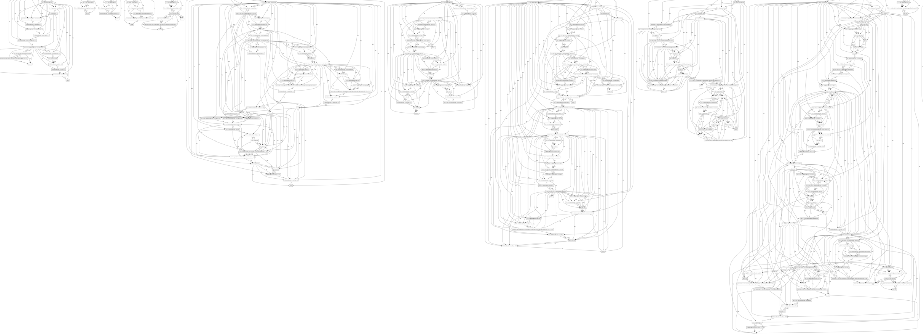
\includegraphics{patterns/reader_pdg_full.png}
%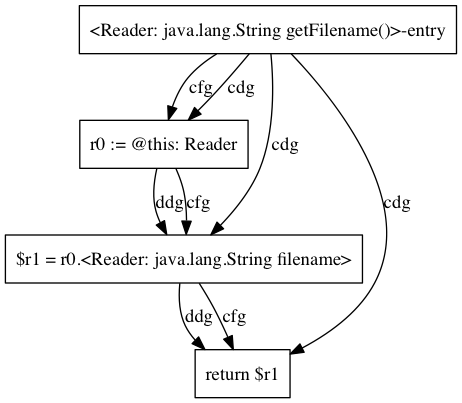
\includegraphics{patterns/reader_getter.png}
%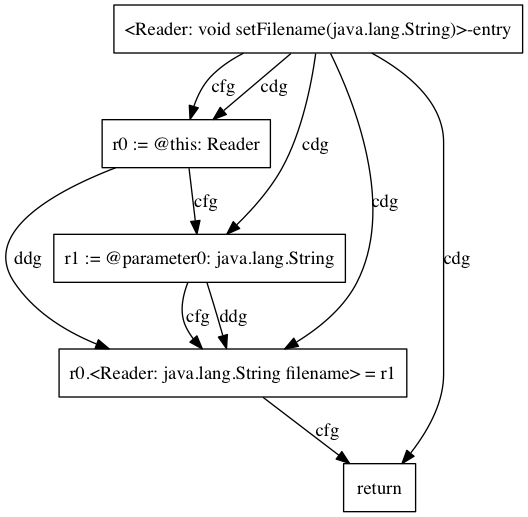
\includegraphics{patterns/reader_setter.png}
%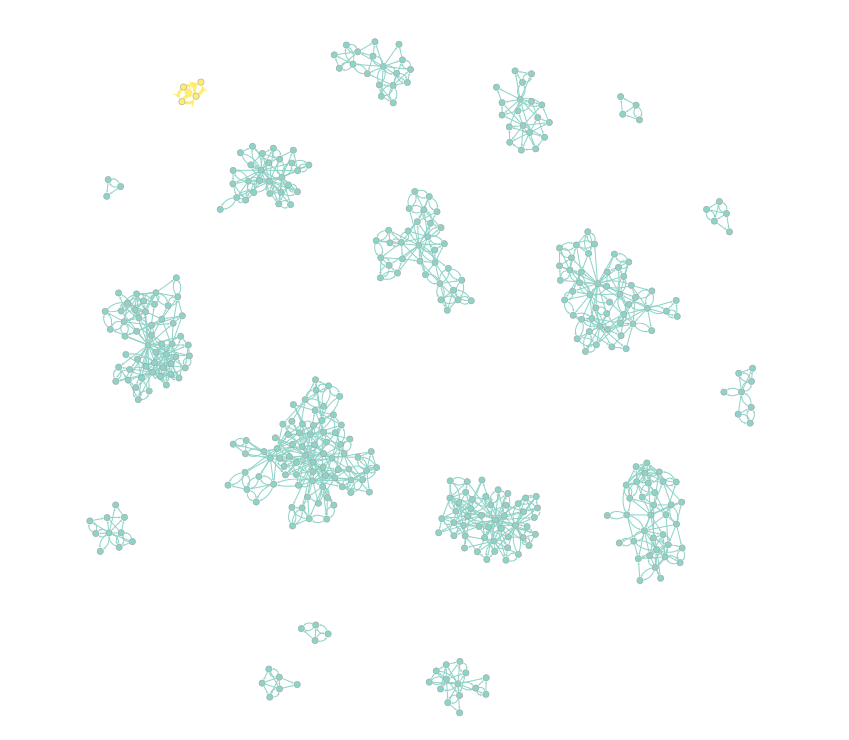
\includegraphics{patterns/reader_getter_isomorphism.png}
%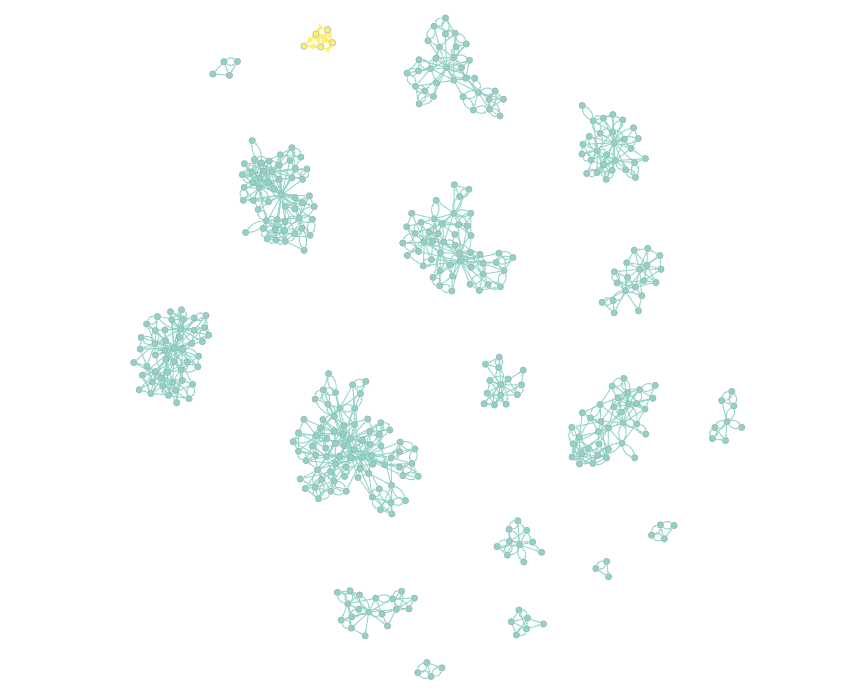
\includegraphics{patterns/reader_setter_isomorphism.png}
%\includegraphics{patterns/full_network.png}
%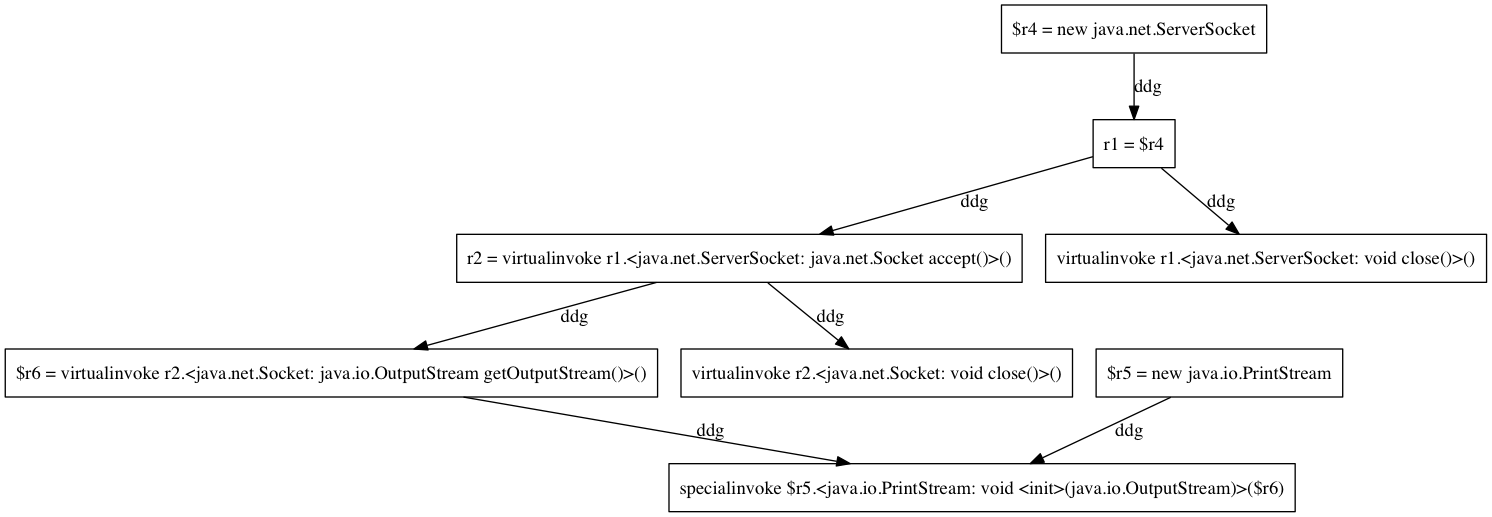
\includegraphics{patterns/networking_pattern.png}
%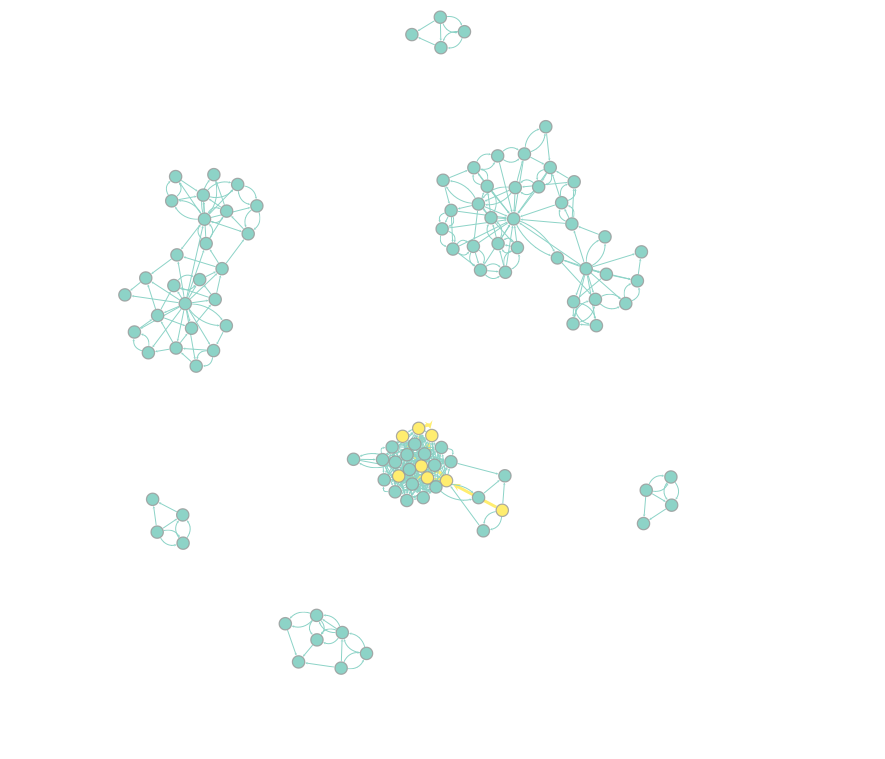
\includegraphics{patterns/networking_isomorphism_full.png}
%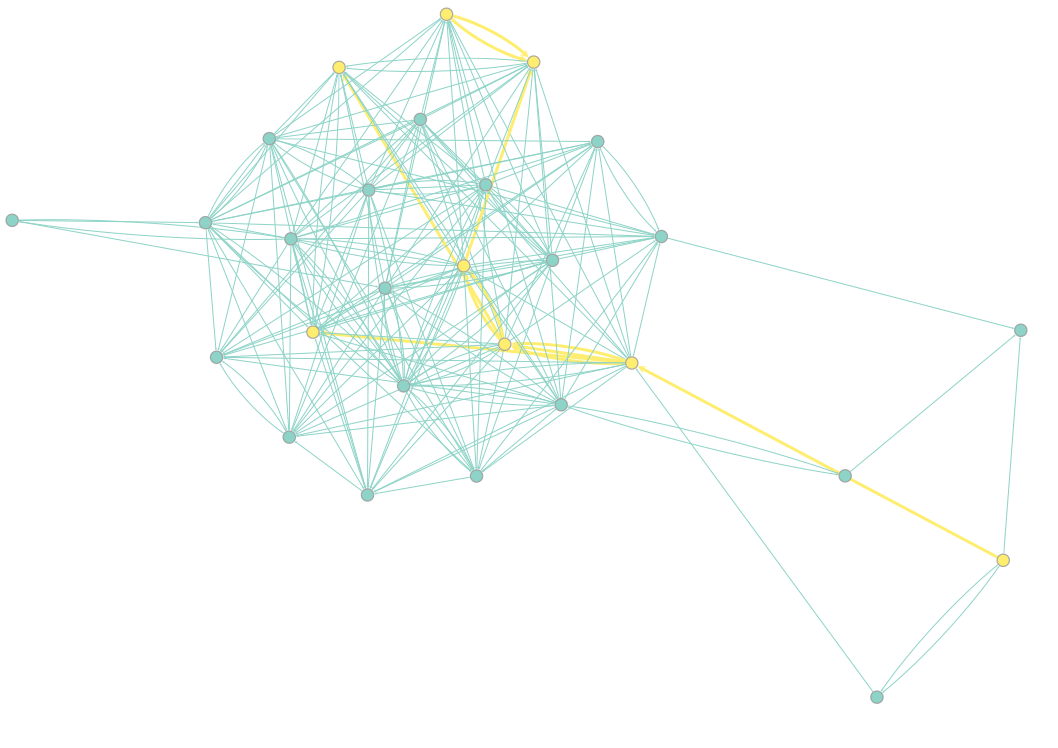
\includegraphics{patterns/networking_isomorphism_zoomed.png}

\section{Conclusion}
pass

\pagebreak
\bibliographystyle{acm}
\bibliography{lit_survey}
\end{document}
